\documentclass[twocolumn]{phdsymp} %!PN
\usepackage[english]{babel}

\usepackage{graphicx}                   % Om figuren te kunnen verwerken
\usepackage{graphics}					% Om figuren te verwerken.
\graphicspath{{figuren/}}               % De plaats waar latex zijn figuren gaat halen.

\usepackage{times}

\hyphenation{}

\def\BibTeX{{\rm B\kern-.05em{\sc i\kern-.025em b}\kern-.08em
    T\kern-.1667em\lower.7ex\hbox{E}\kern-.125emX}}

\newtheorem{theorem}{Theorem}

\begin{document}

\title{Realtime signal synchronization with acoustic fingerprinting} %!PN

\author{Ward Van Assche}

\supervisor{Joren Six, Marleen Denert}

\maketitle

\begin{abstract}
Many experiments executed at IPEM use sensors such as accelerometers and pressure sensors. A common problem after these experiments is the synchronization of data of each sensor. The current synchronization system requires each sensor to be connected to a microphone recording the sound of the environment. With efficient audio-to-audio alignment techniques the latency can be detected very accurately. The current synchronization system is performed as a post-processing step. A real-time and more user-friendly solution is desirable. This paper explores the possibilities to do this. To use the current synchronization algorithms in real-time they had to be changed and optimized in different ways. The new system resulted in a Max/MSP module which makes it possible to run the synchronization in real-time without writing a single line of code.
\end{abstract}

\begin{keywords}
Signal Synchronization, Audio Alignment, Real-Time, Acoustic Fingerprinting, Cross-covariance, Digital Signal Processing
\end{keywords}

\section{Introduction}


\PARstart{E}{xperiments} in various research areas use sensors and video cameras to capture the environment.  Before sensor data and video recordings can be analyzed properly they have to be synchronized accurately in time. This is no easy task because of various reasons. The first problem is that the sensor datastreams can be heterogeneous: the sample rate can vary and the resulted data can be very different (video data or numerical samples). Another difficulty is to cope with the fact that some data sources are unreliable. This can lead to dropped samples and drift which cause unexpected latency changes. The most techniques require a post-processing step: the data has to be synchronized manually or by software \emph{after} the experiment. Because this is impractical and time-consuming a technique which can avoid this is desirable.

The most straightforward way to perform the synchronization is by adding markers. This technique is described in article \cite{bannach2009automatic}. The way how a marker is placed depends on the type of the stream. A short sound can add a marker in an audio stream, a bright flash can do the same in a video stream. The latency can be found by calculating the difference between the marker positions. The usability of this method is limited because of its poor scalability. The synchronization of a large number of streams can be very challenging. Dropped samples and drift can only be detected when the markers are repeated each time interval, which is impractical. The actual synchronization using this technique is only possible as a post-processing step.

Article \cite{jaimovich2010synchronization} describes a method which uses a clock signal to synchronize streams in real-time. However this method avoids the post-processing step it does not fit the requirements: each device (sensor, video camera) should accept a clock-signal as input. Because these devices are very expensive this method is not feasible for the stated problem.

Article \cite{six2015multimodal} discusses a similar problem where its approached in an entirely different way. The described method does not try to synchronize the streams directly. Instead, the (recorded) environment sound is embedded in each stream. This ploy reduces the initial problem to audio-to-audio alignment. Because the recorded environment sound is almost the same for each stream the problem is much easier to tackle. The audio-to-audio algorithms described in the article perform very well. The latency can be detected with a precision less than 1ms. However the article only describes a post-processing approach, the used algorithms look very interesting.

The next part of this paper will describe a method to synchronize streams in real-time using the algorithms mentioned in the previous article. The word ``real-time'' can be ambiguous in a signal-processing context. Therefore it's important to specify some requirements for a real-time system. Because the latency-detecting algorithms need some amount of audio in order to determine the latency it's impossible to immediately output the synchronized signals. In this paper the real-time restriction refers to the fact that the synchronization algorithms are executed while the sensors are collecting data. The post-processing step should be avoided.

\section{Determining latency}

The method described in article \cite{six2015multimodal} uses two latency detecting algorithms which are very complementary. By combining them, latency can be detected very accurately.

\subsection{Acoustic fingerprinting}
Acoustic fingerprinting is a fast and robust technique for comparing audio fragments initially described in article~\cite{Wang2003a}. The technique uses fingerprints based on spectral peaks. Each fingerprint contains condensed information based on typical audio properties. This technique allows finding similar audio fragments ignoring noise and other disturbing background sounds. 

However the initial application was identifying an audio recording using a huge database containing a myriad of fingerprints it's also possible to compare the fingerprints of recordings mutually. The latency can be detected by calculating the offset between the fingerprints. The precision varies around 16~ms to 32~ms, this depends on the used parameters.

\subsection{Calculating the cross-covariance}
The cross-covariance (also referred to as cross-correlation) is a calculation which measures the degree of similarity between two time sequences. Because an audio signal is a time sequence this calculation can be used for determining the latency. When the cross-covariance value is calculated for each possible shift between two audio fragments the shift with the highest result determines the latency.

This method can determine the latency to the nearest sample. The precision in milliseconds depends on the sample rate: when the sample rate is 8000~Hz the maximum precision is $ 1/8000~\textrm{Hz} = 0.125~\textrm{ms} $.

A disadvantage to this method is its performance. The time complexity of the algorithm is $ O(n^2) $ where $ n $ is the number of samples in each signal. Finding the latency between two audio fragments of 10~s at a sample rate of 8000~Hz would asymptotically result in $ 6.4 \cdot 10^9 $ calculations, which is unfeasible on a regular computer. 

\subsection{Refining the results}

The two previously described algorithms are very complementary. Acoustic fingerprinting allows finding the latency very fast and robustly. The cross-covariance algorithm can detect the latency between two tiny pieces of audio very accurately. These advantages can be easily combined.

By determining the raw latency with acoustic fingerprinting, the number of samples used in the cross-covariance calculation can be limited. By cutting the raw latency from the corresponding audio fragment, the new latency is reduced. When the acoustic fingerprinting algorithm uses a precision of 32~ms, the cross covariance should be calculated on two audio fragments of at least 256 samples (when the sample rate is 8000~Hz). This asymptotically results in $65\,536$ calculations, which is much more feasible than without the acoustic fingerprinting step.

\section{Buffering streams}
Sed nec tortor in libero rutrum pellentesque\cite{six2014tarsosdsp} et gravida turpis. Phasellus gravida neque vitae elit fringilla, a efficitur purus sollicitudin. Proin lacus est, suscipit sed nibh ac, hendrerit eleifend leo.
%Schrijven dat het noodzakelijk is om streams te bufferen alvorens het mogelijk is om de synchronisatie in realtime uit te voeren.

\section{Latency filters}
Sed nec tortor in libero rutrum pellentesque\cite{six2014tarsosdsp} et gravida turpis. Phasellus gravida neque vitae elit fringilla, a efficitur purus sollicitudin. Proin lacus est, suscipit sed nibh ac, hendrerit eleifend leo.
%Schrijven over het feit dat omdat alles realtime gebeurt het moeilijker is om handmatige foutcorrectie te doen. Dat er daarom een moving median filters eventueel foutieve pieken kan wegfilteren.

\begin{figure}[ht]
	\begin{center}
		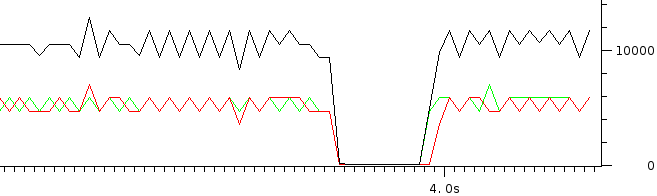
\includegraphics[width=.40\textwidth]{referentie-detail}
		\caption{\label{2AP}Detailed capture of the stream at the moment of a handover between two simulated AP's with a strong signal.  Notice the gap of 100~ms.}
	\end{center}
\end{figure}

\section{Synchronization}
Sed nec tortor in libero rutrum pellentesque\cite{six2014tarsosdsp} et gravida turpis. Phasellus gravida neque vitae elit fringilla, a efficitur purus sollicitudin. Proin lacus est, suscipit sed nibh ac, hendrerit eleifend leo.
%Schrijven over hoe de latencies kunnen worden omgezet zodat het mogelijk is om streams te synchroniseren zonder extra samples te verliezen.

\section{Results}
Sed nec tortor in libero rutrum pellentesque\cite{six2014tarsosdsp} et gravida turpis. Phasellus gravida neque vitae elit fringilla, a efficitur purus sollicitudin. Proin lacus est, suscipit sed nibh ac, hendrerit eleifend leo.
%Schrijven over de Max/MSP module, de mogelijkheid om de synchronisatie met de Teensy microcontroller uit te voeren. TeensyReader en Sync module omschrijven.

\section{Conclusion}
Sed nec tortor in libero rutrum pellentesque\cite{six2014tarsosdsp} et gravida turpis. Phasellus gravida neque vitae elit fringilla, a efficitur purus sollicitudin. Proin lacus est, suscipit sed nibh ac, hendrerit eleifend leo.
%Schrijven over wat er in de toekomst nog verwezenlijkt kan worden. Terugblik naar introductie, schrijven over videostreams en MIDI

\bibliographystyle{phdsymp}
\bibliography{../bronnen/bronnen}

\end{document}
